\documentclass[tikz,border=10pt]{standalone}
\usepackage{amsmath}
\usepackage{amssymb}
\usetikzlibrary{positioning, arrows.meta, shapes.geometric, calc, fit, backgrounds}

\begin{document}
	
	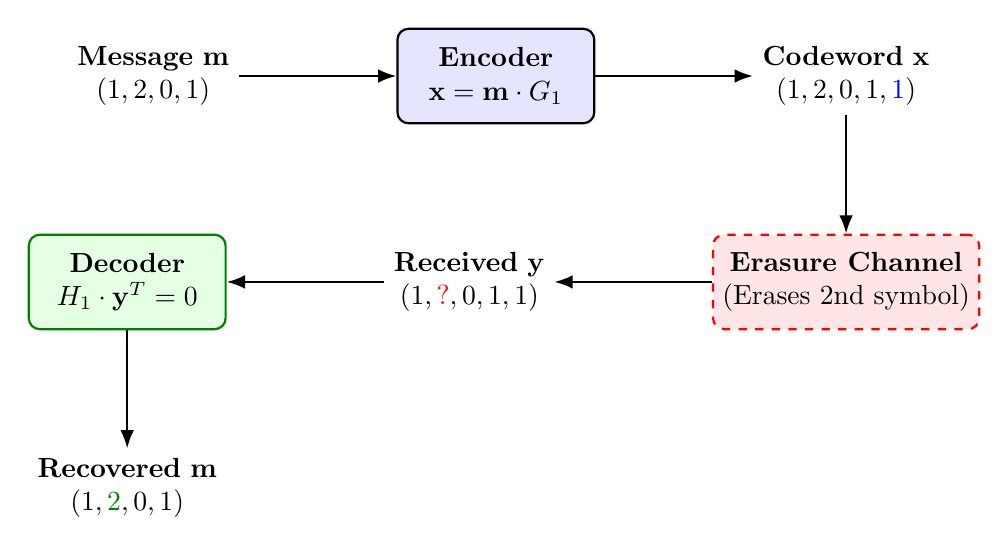
\begin{tikzpicture}[
		>=stealth,
		node distance=1.5cm and 2cm,
		block/.style={draw, rectangle, minimum height=1.2cm, minimum width=2.5cm, align=center, fill=blue!5, rounded corners, thick},
		mathmat/.style={matrix of math nodes, left delimiter=(, right delimiter=), inner sep=2pt, column sep=0.15cm},
		arr/.style={->, thick, >=Latex},
		highlight/.style={text=red, font=\bfseries}
		]
		
		% 1. Source Message
		\node (msg) [align=center] {\textbf{Message} $\mathbf{m}$ \\ $(1, 2, 0, 1)$};
		
		% 2. Encoder
		\node[block, fill=blue!10] (enc) [right=of msg] {\textbf{Encoder} \\ $\mathbf{x} = \mathbf{m} \cdot G_1$};
		
		% 3. Codeword
		\node (codeword) [align=center, right=of enc] {\textbf{Codeword} $\mathbf{x}$ \\ $(1, 2, 0, 1, \color{blue}1\color{black})$};
		
		% 4. Channel
		\node[block, fill=red!10, dashed, draw=red] (channel) [below=of codeword] {\textbf{Erasure Channel} \\ (Erases 2nd symbol)};
		
		% 5. Received Vector
		\node (received) [align=center, left=of channel] {\textbf{Received} $\mathbf{y}$ \\ $(1, \color{red}?\color{black}, 0, 1, 1)$};
		
		% 6. Decoder
		\node[block, fill=green!10, draw=green!50!black] (dec) [left=of received] {\textbf{Decoder} \\ $H_1 \cdot \mathbf{y}^T = 0$};
		
		% 7. Recovered Message
		\node (recovered) [align=center, below=of dec] {\textbf{Recovered} $\mathbf{m}$ \\ $(1, \color{green!50!black}2\color{black}, 0, 1)$};
		
		% Arrows for the main flow
		\draw[arr] (msg) -- (enc);
		\draw[arr] (enc) -- (codeword);
		\draw[arr] (codeword) -- (channel);
		\draw[arr] (channel) -- (received);
		\draw[arr] (received) -- (dec);
		\draw[arr] (dec) -- (recovered);
		
		% 8. Explanation Box for the Math
%		\node[draw, rectangle, rounded corners, fill=yellow!10, text width=6.5cm, align=left, right=of dec, xshift=0.5cm, yshift=-1cm] (math) {
%			\textbf{Recovery Math (over $\mathbb{F}_3$):} \\[1ex]
%			Parity Check Matrix:\\ 
%			$H_1 = (2, 2, 2, 2, 1)$ \\[1ex]
%			Equation $H_1 \cdot \mathbf{y}^T = 0$:\\
%			$2(1) + 2({\color{red}x_2}) + 2(0) + 2(1) + 1(1) = 0$ \\[1ex]
%			Simplify modulo 3:\\
%			$2 + 2{\color{red}x_2} + 0 + 2 + 1 \equiv 0 \pmod 3$ \\
%			$2{\color{red}x_2} + 5 \equiv 0 \pmod 3$ \\
%			$2{\color{red}x_2} + 2 \equiv 0 \pmod 3$ \\[1ex]
%			Solve for ${\color{red}x_2}$:\\
%			$2{\color{red}x_2} \equiv -2 \equiv 1 \pmod 3$ \\
%			Multiply both sides by 2 (inverse of 2 in $\mathbb{F}_3$):\\
%			${\color{red}x_2} = \mathbf{2}$
%		};
		
%		\draw[arr, dashed, color=gray] (dec) |- (math);
		
%		% Title6
%		\node[align=center, font=\Large\bfseries] at ($(enc)!0.5!(channel) + (0, 3cm)$) {Single Erasure Correction over $\mathbb{F}_3$ ($n=5, k=4$)};
		
	\end{tikzpicture}
	
\end{document}